\chapter{Paquete \trm}\label{sec:transmem66i}

\section{Introducción}
El tratamiento de datos para la obtención de resultados numéricos y gráficos es un paso muy importante en el estudio de todos los sistemas. Los procesos de transporte estudiados en el presente trabajo no generan una gran cantidad de datos y su tratamiento no es particularmente complicado. En muchos lugares, estas tareas se cumplen usando herramientas como hojas de calculo que realmente no fueron diseñadas para su aplicación en ciencias exactas. El uso de programas como Microsoft Excel\textregistered\ la mayoría de las veces no acarrea consecuencias negativas en los resultados obtenidos, pero muchos de los procedimientos deben ser llevados a cabo siguiendo protocolos tediosos que involucran mucho trabajo {manual} que disminuye sus capacidades de reusabilidad y adaptabilidad \citep{Incerti2019}. Los gráficos generados por defecto en este tipo de plataformas distan de los conceptos de la gramática de los gráficos \citep{Wilkinson2005}. 

Existen múltiples alternativas más apropiadas que se encuentran basadas en lenguajes de programación modernos que ganan cada vez más popularidad. Entre las muchas ventajas que presentan estos lenguajes, está que la mayoría de las veces son de código abierto y eso asegura su disponibilidad para todas las personas, sin importar el presupuesto que tengan asignado para su investigación. Su uso involucra un gasto computacional mucho menor, por lo que análisis muy poderosos pueden hacerse en tiempos cortos empleando computadoras muy convencionales. Estas alternativas son altamente potencializables por medio de librerías o {paquetes} que son un conjunto de funciones pensadas para resolver una serie de problemas particulares. Un gran número de paquetes se encuentran disponibles y los números van en aumento. Los lenguajes de programación de código abierto exitosos generan una gran comunidad de usuarios y desarrolladores, dispuestos a brindarse ayuda mutua a través de diversas plataformas como \url{https://stackoverflow.com/}.


\R\ es un entorno de programación que permite computación estadística y representación gráfica de datos \citep{R}. Una excelente introducción a \R\ fue escrita por \citet{Venables2004}. \R\ se encuentra disponible para la mayoría de los sistemas operativos comunes y está constantemente bajo actualización y mejora. El repositorio oficial \ac{CRAN} contiene más de 15000 librerías plenamente documentadas y disponibles para cualquier persona con acceso a internet. Existen numerosos paquetes de gran utilidad para distintas ramas de la química. Algunos ejemplos importantes se muestran en la Tabla \ref{tab:Rpackages}.

\begin{table}[H]
    \centering\footnotesize
    \begin{tabular}{@{}lp{9.55cm}l@{}}\toprule
        \textbf{Nombre} & \textbf{Propósito} & \textbf{Referencia} \\\midrule
         \verb|chemometrics|&Análisis estadístico multivariado en quimiometría &\citet{Filzmoser2017}\\
         \verb|propagate|&Propagación de incertidumbre &\citet{Spiess2018}\\
         \verb|FrF2|&Creación y análisis de diseños factoriales fraccionados de dos niveles &\citet{FrF2}\\
         \verb|rsm|&Métodos de análisis de respuesta& \cite{Lenth2009}\\
         \verb|DoE.base|&Diseños factoriales fraccionados &\citet{Gromping2018}\\
         \verb|eChem|&Simulación de experimentos de electroquímica &\citet{Harvey2015}\\
         \verb|spectral|&Métodos comunes en el análisis de datos espectrales &\citet{SeilMayer2019}\\
         \verb|ChemoSpec|&Quimiometría exploratoria para espectroscopía &\citet{Hanson2020}\\
         \verb|AFM|&Análisis de imágenes de microscopía de fuerza atómica &\citet{Beauvais2019}\\
         \verb|SixSigma|&Herramientas \textit{seis sigma} para control de calidad y mejora continua &\citet{Cano2015}\\
         \verb|RGCxGC|&Análisis de datos bidimensionales de cromatografía de gases&\cite{Quiroz2020}\\
         \verb|labsimplex|&Algorítmos de optimización simplex para aplicaciones de laboratorio$^a$&\citet{labsimplex}\\\bottomrule
         \multicolumn{3}{@{}l@{}}{$^{a.}$\scriptsize Paquete aún no disponible en CRAN. La versión beta puede descargarse de \url{https://github.com/Crparedes/labsimplex}}
    \end{tabular}
    \caption{Ejemplos de paquetes de R diseñados para distintas áreas de la química.}
    \label{tab:Rpackages}
\end{table}

Se escribieron y documentaron distintas funciones en \R\ para automatizar el tratamiento de los numerosos conjuntos de datos generados durante el presente trabajo de investigación. Estas funciones fueron posteriormente aglomeradas en el paquete \trm. En el paquete se incluyeron algunos conjuntos de datos que fueron producidos durante algunos de los experimentos realizados para ilustrar el uso de las funciones. El manual oficial del paquete se encuentra en el Anexo \ref{sec:transmemManual}. El código fuente del paquete puede encontrarse en el repositorio \url{https://github.com/Crparedes/transmem}. A pesar del gran número de librerías disponibles en \ac{CRAN}, hasta donde sabemos, no existe aún ninguna librería disponible para el tratamiento de datos provenientes de procesos de transporte a través de membranas.

En este capítulo se esquematiza el uso general del paquete y se describe su proceso de instalación. Los detalles de las funciones pueden ser encontradas en el manual oficial donde se encuentran ejemplos prácticos que hacen uso de los conjuntos de datos mencionados.

%La información que se alimenta a las funciones de \trm en la mayoría de los casos puede ser cargada desde un archivo de texto plano o ingresada manualmente dependiendo de las características de los instrumentos empleados. En el presente capítulo se ha optado por el segundo enfoque el cual, a pesar de sus limitaciones prácticas, ofrece un panorama más claro y reproducible para quien desee aprender a usar el paquete desde ceros. Para más detalles sobre cómo cargar datos desde archivos vea el Capítulo 7 del libro de \cite{Venebles2004}.
\clearpage
\section{Instalación del paquete}
\enlargethispage{1\baselineskip}
Antes de instalar \trm\ es necesario tener instalado \R\ en una versión igual o superior a la 3.5.0. Se recomienda adicionalmente la instalación de Rstudio (\url{https://rstudio.com/}) que es una \ac{GIU} diseñada para facilitar grandemente el trabajo de datos con \R. 

El paquete ha sido aceptado en el repositorio oficial \ac{CRAN}. La ultima versión oficial puedeinstalarse con el comando general:
\begin{lstlisting}[belowskip=-2.6\baselineskip]
install.packages('transmem')
\end{lstlisting}

La última versión construida del paquete\footnote{El recibe actualizaciones regularmente.} \trm\ puede descargarse directamente desde su repositorio en Github uśando el paquete \verb|devtools| \citep{Hadley2019}:
\begin{lstlisting}[belowskip=-2.6\baselineskip]
if (!require("devtools")) install.packages("devtools")
devtools::install_github("Crparedes/transmem")
\end{lstlisting}


Si el paquete ha sido instalado correctamente aparecerá en la pantalla de comandos de \R:
\begin{lstlisting}
#    > Installing package into '/home/cris/R/x86_64-pc-linux-gnu-library/3.6'
#    >   (as 'lib' is unspecified)
#    > * installing *source* package 'transmem' ...
#    > ** using staged installation
#    > ** R
#    > ** data
#    > *** moving datasets to lazyload DB
#    > ** byte-compile and prepare package for lazy loading
#    > ** help
#    > *** installing help indices
#    > ** building package indices
#    > ** testing if installed package can be loaded from temporary location
#    > ** testing if installed package can be loaded from final location
#    > ** testing if installed package keeps a record of temporary installation path
#    > * DONE (transmem)
\end{lstlisting}
El paquete estará listo para ser cargado en el ambiente de trabajo para poder usar sus funciones:

\begin{lstlisting}[belowskip=-2.6\baselineskip]
library('transmem')
\end{lstlisting}

\clearpage
\section{Operación del paquete}
La Figura \ref{fig:chap4esquema} contiene el esquema de las funciones principales del paquete. En el mapa conceptual se sugiere una secuencia inicial de tres pasos pensada para transformar los datos experimentales al formato apropiado para las funciones del paquete. La matriz de datos del transporte contiene la concentración o la fracción de una especie en función del tiempo en ambas disoluciones (alimentación y recuperación). Esta matriz (que es en realidad un \textit{data.frame}) es la que se usa para producir los resultados numéricos y generar las representaciones gráficas pertinentes.

{\floatstyle{boxed}
\restylefloat{figure}
\begin{figure}[H]
    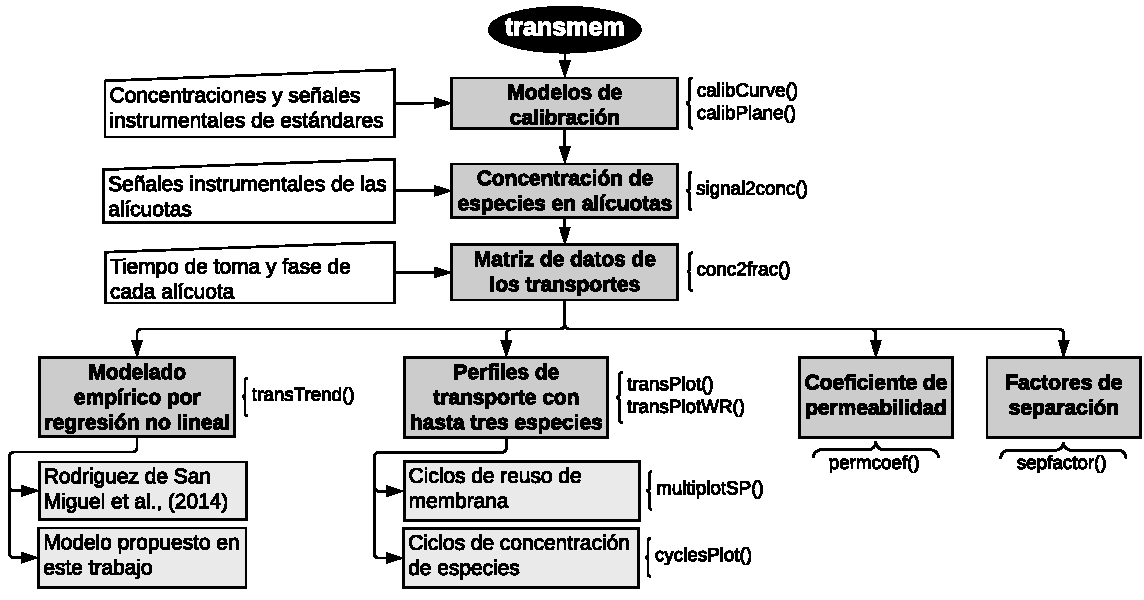
\includegraphics[width=\textwidth]{chap4/Chapter4Thesis.pdf}
    \caption{Esquema de las funciones principales del paquete \trm.}
    \label{fig:chap4esquema}
\end{figure}
}

Para conocer como se usa alguna función se recomienda ver el manual de referencia del paquete en el Anexo \ref{sec:transmemManual}. Una alternativa es usando la función \verb|help()| luego de haber cargado el paquete. Para ver la ayuda de una función en particular, escriba en la ventana de comandos de \R: 
\begin{lstlisting}
help("nombre_de_la_funci\'on")
\end{lstlisting}

La interfaz gráfica de la aplicación web se encuentra en desarrollo y se está buscando un servidor oficial en la Facultad para ponerlo a disposición de la comunidad. Mientras el espacio en el servidor es asignado, la aplicación puede ser utilizada (con algunas limitantes) en la página \url{https://crparedes.shinyapps.io/transmem_shinyapp/}.
\clearpage
\ChapBib{chap4/Chap4}
%\section{Creación de modelos de calibración}
%Monitorear la concentración de una especie en función del tiempo es fundamental en muchos procesos de transporte a través de membranas. Esto por lo general involucra la comparación de las señales que producen las muestras en respuesta a un estímulo para compararlas con las producidas por disoluciones estándar de concentración conocida. La comparación se hace por métodos de regresión que involucran curvas de calibración y eventualmente, planos de calibración, entre otros. Para crear una curva de calibración debe conocerse la concentración de la especie de interés y la señal producida por la misma para cada estándar. 

%\begin{lstlisting}[belowskip=-2.6\baselineskip]
%curvelithium <- data.frame(conc   = c(0.00, 0.05, 0.23, 0.73, 0.92, 1.30, 1.66, 2.11),
%                           signal = c(0.000, 0.036, 0.162, 0.477, 0.586, 0.797, 0.971, 1.169))
%lithiummodel <- calibCurve(curvelithium, order = 2)
%\end{lstlisting} 

%Se genera un gráfico con la información de la curva de calibración. El gráfico se muestra en la Figura \ref{fig:calcurvetrm1}(a). El comando \verb|plot(lithiummodel$residuals)| hace el gráfico de residuales de la regresión para evaluar la pertinencia del modelo escogido, este gráfico se muestra en la Figura \ref{fig:calcurvetrm1}(b). Para visualizar en detalle el modelo generado, la significancia estadística de cada parámetro y la significancia estadística de toda la regresión se usa la función \verb|summary()|. 
%\begin{lstlisting}[belowskip=-2.6\baselineskip]
%summary(lithiummodel)
%#      > Call:
%#      > lm(formula = Signal ~ Conc + I(Conc^2), data = curveN)
%#      > 
%#      > Residuals:
%#      >          1          2          3          4          5          6          7... 
%#      > -0.0014330 -0.0003988  0.0026637  0.0003075 -0.0019808  0.0018193 -0.0015631...
%#      > 
%#      > Coefficients:
%#      >              Estimate Std. Error t value Pr(>|t|)    
%#      > (Intercept)  0.001433   0.001293   1.108    0.318    
%#      > Conc         0.702864   0.003280 214.264 4.20e-11 ***
%#      > I(Conc^2)   -0.070992   0.001589 -44.674 1.06e-07 ***
%#      > ---
%#      > Signif. codes:  0 '***' 0.001 '**' 0.01 '*' 0.05 '.' 0.1 ' ' 1
%#      > 
%#      > Residual standard error: 0.001971 on 5 degrees of freedom
%#      > Multiple R-squared:      1,	Adjusted R-squared:      1 
%#      > F-statistic: 1.725e+05 on 2 and 5 DF,  p-value: 7.995e-13
%\end{lstlisting} 

%En algunos casos, más de una variable explicatoria debe ser considerada en la respuesta instrumental de un equipo. Por ejemplo, la señal de absorción de litio por \ac{FAAS} se ve intensificada por la presencia de sodio en la muestra (ver Sección Anexa \ref{sec:planar1}). Un modelo bivariado (i.e.\ planar) es la opción más adecuada y la forma de generarlo es similar al mostrado anteriormente solo que debe incluírse un segundo vector de concentraciones con los datos de la segunda variable explicatoria que debe ser considerada. La función que debe usarse es \verb|calibPlane|.

%Los objetos creados \verb|lithiummodel| y \verb|planemodel| pueden ser utilizados para interpolar señales de muestras con el propósito de 

%\section{Fracciones transportadas y modelamiento empírico de perfiles}